\documentclass[urop]{nurop}
\usepackage{fullpage}
\usepackage{amsmath}
\usepackage{amssymb}
\usepackage{graphicx}
\usepackage[ruled,vlined]{algorithm2e}
\graphicspath{{./images/}}
\begin{document}

\newcommand{\A}{\mathcal{A}}
\newcommand{\R}{\mathcal{R}}
\newcommand{\W}{\mathcal{W}}

\title{CP3208 Undergraduate  \\
	Online Task Assignment\\
	Progress Report}

\author{\large{Tan Wei Yang} \\ A0173236H \\ 
	\normalsize\textit{Department of Computer Science,\\
	School of Computing,\\
	National University of Singapore} 
}
\maketitle


\section{Introduction}
This is a progress report for the project on online task assignment. First, we introduce the specific variant of online task assignment. Next, we recap existing literature on online task assignment, as well as other related problems, and how the work done can be applied to this project. Then, we cover the work that has been done on this project. Finally, we give an outline of the plan for CP3209, the continuation of this project.

\subsection{Motivation}
Online task assignment is a ubiquitous problem. From courier services to transport systems that utilize crowdsourcing like Grab, we require algorithms to assign service providers to users. We ultimately focus on the context of a firm that hires a fleet of service providers to satisfy requests from users, similar to a taxi or a delivery company. In this context, the service provided consists of moving a person or object from a start location to an end location. A major source of operational costs for firms providing such services is the cost of hiring a fleet of workers to meet service requests. Hence, we ultimately seek to minimize the size of the fleet, while keeping to certain constraints. The constraint we have decided to look at is a maximum delay between the time of creation of a service request and the time at which a worker starts to fulfil the request. This is akin to providing a guarantee on the maximum waiting time.



\section{Review of Literature}
\label{lit}
In this section, we look at various problems that are related to the minimum fleet problem. For each problem, we will give an overview of the theoretical results and algorithms in the literature that are relevant to the minimum fleet problem, as well as any experimental evaluation performed. 

\subsection{Minimum Fleet Problem}
To the best of our knowledge, our exact formulation of the minimum fleet problem is not well studied. \cite{nature} presents an offline algorithm for a variant of the minimum fleet problem, and uses the results as a benchmark to analyse two online algorithms.

\subsubsection{The Offline Problem}
Instead of a maximum delay constraint, \cite{nature} imposes a zero delay constraint, as well as a maximum connection time, $\delta$, for their offline variant of the minimum fleet problem. Connection time refers to the time between completing a request and starting the next request. This can also be seen as the amount of time the worker is idle for. 

\subsubsection{Shareability Graph}
\cite{nature} solves the above offline minimum fleet problem in using a directed graph structure known as the shareability graph.

The vertices of the shareability graph represent requests and an edge from request $r_i$ to request $r_j$ indicates that $r_j$ can be assigned to the same worker consecutively after $r_i$ without violating the maximum connection time $\delta$ with zero delay.

This transforms the minimum fleet problem into a minimum path cover problem, where the minimum number of workers required is exactly the minimum number of paths.

The resulting shareability graph is a directed acyclic graph as $t_{r_i} < t_{r_j}$ for all edges $(r_i, r_j)$ in the graph, inducing a natural topological order. Hence, the equivalent minimum path cover problem can be solved efficiently using the Hopcroft-Karp algorithm.

The value of $\delta$ used has to be set by the service operator, and needs to be tuned to the dataset.  

\subsubsection{Online Algorithms}
\cite{nature} further presents two online algorithms for task assignment.

\vspace{2mm} \noindent \textbf{On-the-fly Assignment}

\noindent For each request $r$ that is made, the first available vehicle that minmizes waiting time is chosen.

\vspace{2mm} \noindent \textbf{Batch Assignment}

\noindent Requests are collected over fixed time intervals and processed in batches. For each batch, maximum bipartite matching is used to assign workers to requests. The matching is done to maximise the number of trips that can be fulfilled within a fixed delay.

\subsubsection{Comparison with Real-World Data}
The performance of the offline and online algorithms were compared against a dataset consisting of all taxicab trips in New York City in 2011. A street network of Manhatten was first constructed using open data of the map, and travel times are computed using historical data. The details of the preprocessing and travel time computation are based on the supplementary information from \cite{preprocess}. 

Compared to the actual dataset, the minimum fleet size obtained by constructing the shareability graph for daily demand was 40\% lower than the actual number of circulating taxis. The batch assignment achieved a 30\% reduction in fleet size while fulfilling a maximum delay of 6 minutes for more than 90\% of trip requests, which is close to the 40\% achieved by the offline method. The batch assignment consistently had a higher percentage of trips served while fulfilling the maximum delay compared to the on-the-fly model.

\subsubsection{Discussion}

\vspace{2mm} \noindent \textbf{Use of Offline Minimum for Comparison}

\noindent We note that while the performance of batch assignment seems optimistic when compared to the offline lower bound, the lower bound obtained from the shareability graph is not entirely analogous to the result of online assignment. The offline assignment does not allow for any request to have any delay, in addition to the connection time constraint. These conditions are much stronger than the conditions for online assignment.

However, it is difficult to obtain a more suitable lower bound that allows for the same level of service guarantees as the online assignment. In particular, shareability graph cannot be easily modified to allow for delays. Due to the cumulative nature of delays, whether or not two requests can be fulfilled consecutively depends not only on the attributes of each request, but also the delay experienced by the first trip. Hence, the presence of an edge depends on the path taken.

\vspace{2mm} \noindent \textbf{Comparison between Online Algorithms}

\noindent Batch assignment was shown to consistently have a higher percentage of trips served within the maximum delay compared to the on-the-fly assignment, which is reasonably within expectation, as the maximum matching in batch assignment is optimised for the maximum delay.

However, depending on the nature of the exact application, we may also need to pay attention to catastrophic delays in requests that are not served while fulfilling the maximum delay.

\subsection{Batch-based Maximum Bipartite Matching}
In the literature for spatial crowdsourcing, maximum bipartite matching is often used to find the maximum number of requests that can be served in each batch of requests. This is in line with the minimum fleet problem, which seeks to fulfill all (or most) requests with a maximum delay constraint. In this section, we present algorithms presented by \cite{kazemi} for batch-based maximum bipartite matching.

\subsubsection{Greedy Algorithm for Batch-Based Assignment}
In the greedy algorithm, for each batch, the optimal assignment for the batch is taken. In other words, the assignment serves the maximum number of requests possible for the batch. This is done by reducing the problem into a maximum flow problem, by connecting worker vertices to request vertices that it can fulfill. After constructing the flow network graph, any algorithm for solving the maximum flow problem, such as the Ford-Fulkerson algorithm, can be applied to obtain an optimal solution for thee batch. 

\subsubsection{Least Location Entropy Priority}
\label{llep}
As the greedy algorithm does not take into account long term performance, \cite{kazemi} devised an algorithm (G-llep) using a heuristic, where requests that are located in worker-sparse areas are given greater priority as they are less likely to be fulfilled. This is done by calculating location entropy for each discretized location, which involves the proportion of visits each worker made to that location. By associating each request with its location entropy, the problem is reduced to a minimum-cost maximum flow problem, which can be solved by applying linear programming to the maximum flow result.

\subsubsection{Nearest Neighbour Priority}
\cite{kazemi} also presents another algorithm (G-nnp) that uses a heuristic to minimize the total travel cost. A similar approach to section~\ref{llep} is used, except the weights in the minimum-cost maximum flow problem are the distances between the requests and the workers instead.
\label{nnp}

\subsubsection{Experimental Comparison}
\cite{kazemi,cheng} both performed experimental evaluation of these 3 algorithms on synthetic data following uniform distribution of worker and request locations. In addition, \cite{kazemi} used real data from Gowalla, an application that allows users to check into locations they have visited; \cite{cheng} uses data of the temporal locations of taxis and orders between 7.30a.m. and 8.30a.m. in a normal day in urban Beijing, obtained from DiDi Chuxing.

For both studies, G-llep consistently produces better results than the greedy algorithm in terms of number of requests fulfilled, whereas G-nnp performs worse than the greedy algorithm under the same metric, but performs better in terms of average travel cost.  
\label{nnpexp}

\subsubsection{Discussion}
\label{discussion}
As expected, G-llep performs better than the greedy algorithm. However, location entropy may not be directly used in the minimum fleet problem. We require all reqests to be assigned with a maximum delay, and the concept of prioritizing requests under such a strong condition seems redundant. However, we can still adapt the idea of incorporating knowledge of the distribution of workers into our algorithm.

\subsection{Online Maximum Bipartite Matching}
In this section, we look at the algorithms and theoretical results for online maximum bipartite matching presented by \cite{karp,goel}
\subsubsection{Deterministic Algorithms}
\cite{karp} proves that any deterministic algorithm for online maximum bipartite matching can only have a competitive ratio of up to $\frac{1}{2}$ under the adversarial model. \cite{goel} proves that the competitive ratio has an upper bound of $\frac{3}{4}$ in a random order model.

\vspace{2mm} \noindent \textbf{GREEDY Algorithm}

\noindent \cite{karp} shows that the GREEDY algorithm, where a request is matched to an arbitrary worker that can fulfill it as long as it is possible (the alternative being to not match it), achieves the upper bound competitive ratio of $\frac{1}{2}$ under the adversarial model, as well as a competitive ratio of $1 - \frac{1}{e}$ under the random order model.

\subsubsection{Randomized Algorithms}
\cite{karp} proves that the competitive ratio for any online algorithm in the adversarial model has an upper bound of $1 - \frac{1}{e}$.
\cite{goel} proves that the competitive ratio of any randomized algorithm has an upper bound of $\frac{5}{6}$ in a random order model.

\vspace{2mm} \noindent \textbf{RANKING}

\label{ranking}
\noindent \cite{karp} presents the RANKING algorithm, which first generates a random permutation among all workers. The workers are given priority based on this permutation. When a request can be assigned to a worker, the worker of the highest priority is assigned that request.

Although it is simple, this algorithm achieves the optimal competitive ratio of $1 - \frac{1}{e}$ under the adversarial model. Compared to the greedy algorithm, it also achieves a better competitive ratio of 0.696 under the random order model \cite{rankingrandomorder}.

\subsubsection{Discussion}
Relating back to online task assignment, in a small time window, as workers are unlikely to be able to perform more than a single task, the assignment becomes essentially equivalent to online maximum bipartite matching. Hence, the results regarding online maximum bipartite matching could be highly relevant to our study.  

The bounds for competitive ratios under the adversarial and random order models for both deterministic and randomized algorithms suggest that even when there are enough workers for there to exist an optimal assignment, online algorithms are still likely to fail under certain conditions. 

To address this problem, we have to introduce redundancies in our system by increasing the number of workers so that each request can be fulfilled by more workers. In particular, if there are $n$ requests and all requests can be fulfilled by at least $n$ workers, any online algorithm will be able to successfully assign all requests to workers. 

The higher competitive ratio of RANKING in the adversarial and random order models as compared to the greedy algorithm makes it a good candidate for implementation.


\subsection{Online Minimum Cost Maximum Bipartite Matching}
Minimum cost maximum bipartite matching is another problem that is often studied, extending the motivation of the nearest neighbour priority in section~\ref{nnp}. It involves minimizing the cost of .In this section, we will briefly discuss the algorithms in spatial crowdsourcing for minimum weighted matching, as are collated by \cite{tong}.
\subsubsection{Deterministic Algorithms}
\cite{greedy} presents two deterministic algorithms, the greedy, or nearest neighbour algorithm and the permutation algorithm.

The greedy algorithm matches each newly arrived requests with the nearest available worker to minimize cost for each request. \cite{greedy} showed that this results in a competitive ratio of $2^k - 1$ for $k$ workers.

\cite{greedy} also presents another deterministic algorithm, the permutation algorithm, which has an improved competitive ratio of $2k -1$. We will not cover this algorithm in detail.

\cite{tong} argues that while the competitive ratio of the greedy algorithm is bad, under a random order model the worst case scenario presented by \cite{greedy} has a constant competitive ratio of 3.195, and the average case is likely to have a constant competitive ratio as well.

\subsubsection{Randomized Algorithms}
\cite{hst-g} and \cite{hst-re} have respectively presented the HST-Greedy and HST-Reassignment algorithms, which use the $\alpha$-Hierarchically-Separated-Tree ($\alpha$-HST). The randomized nature of both algorithms stem from the construction of the $\alpha$-HST, which is itself a randomized algorithm. The HST-Greedy algorithm takes the nearest available worker to a request, and outputs the worker that is nearest to this worker according to the tree metric. The HST-Reassignment algorithm takes this a step further by allowing for restricted reassignment of previous assignments.

\subsubsection{Experimental Analysis}
\cite{tong} studies the experimental performance of the algorithms introduced in this section, using taxi-calling data on the real-time taxi-calling platform, ShenZhou, for Beijing in May 2015. Additionally, synthetic datasets were generated using various distributions for workers and requests. This includes the Power-Law and Exponential distributions, based on studies that show that the movement of people and taxis usually follow these distributions in cities \cite{dist1,dist2}, as well as the Uniform and Normal distributions, which are commonly used.

For both real and synthetic datasets, the greedy algorithm consistently performed the best, despite its theoretical competitive ratio under the adversarial model. This justifies the belief that the average case competitive ratio for the greedy algorithm should also be constant.

\subsubsection{Discussion}
In general, the algorithms presented here are designed to minimize the total distance travelled. In light of the relatively poorer performance of the nearest neighbour priority heuristic for maximum matching in section~\ref{nnpexp}, the algorithms presented in this section may not be directly applicable to our problem, apart from using the greedy algorithm as a baseline to work with. However, if we are able to model our problem as an online minimum cost maximum bipartite matching, say using a cost metric based on the distribution of workers, we could apply the algorithms discussed in this section.

The experimental analysis by \cite{tong} shows that the theoretical results we obtain from an adversarial analysis does not translate well in experimental evaluation, and analysis from a random-order model would be more suitable.

Furthermore, the experimental setup of \cite{tong} uses a variety of spatiotemporal distributions of workers and requests, which we can consider adopting as well.

\section{Current Progress}
In this section, we discuss the progress that has been made in CP3208. Here, we introduce the prototype model we created, the algorithms implemented and the results we obtained. We then give a brief discussion on the results we have obtained.

\subsection{Prototype Model}
We have implemented a model for online task assignment through object-oriented programming using Python. 

Currently, we are using a 2D Cartesian coordinate to represent locations, and correspondingly Euclidean distance as a distance metric.

We divide data generation, output generation, strategies (algorithms implemented), the overall online task assignment framework, and experimentation with different variables into separate modules.

For each run of online task assignment, a set of workers, a set of requests, a maximum waiting time guarantee, and the assignment strategy are used as inputs.

The results we keep track of are the average waiting time, the maximum waiting time, and the number of requests that did not meet the maximum waiting time guarantee. This is stored in a .csv file, which is then analysed using Microsoft Excel. Additionally, we generate a log of each assignment made in a .txt file.

With the compartmentalization of code, this prototype can be easily extended to include generating data from other distributions, as well as testing other algorithms, with little refactoring. However, the current implementation requires some level of refactoring to be applied to the case where locations are distances are represented in a graph structure. In section~\ref{sec:plan}, we will discuss the plan on how to develop the current prototype.

\subsubsection{Data Generation}
We generate the input locations over a uniform distribution in a unit square, using coordinates $(0,0)$ to $(1,1)$. The time is also generated over a uniform distribution with the range $[0, d]$, where $d$ is the input duration over which requests are generated. 

The workers are generated given an input number of workers to generate. Each worker is assigned a start location under the aforementioned uniform distribution. All workers also have unit velocity (i.e. it takes 1 unit of time to move from $(0,0)$ to $(0,1)$)

The requests are generated given the number of requests to generate, as well as the duration over which the requests are generated as inputs. Each request is assigned a start location, an end location, as well as a creation time based on the distributions mentioned earlier.

\subsubsection{Algorithms Implemented}

In this section, we cover the three algorithms that we have implemented on our prototype. These algorithms are inspired by the algorithms for the related problems covered in section~\ref{lit}

\vspace{2mm} \noindent \textbf{Greedy Algorithm}

\noindent The greedy algorithm essentially assigns the worker that can fulfill the request the earliest. Note that $t_{(w,r)}$ is the waiting time, or delay for the assignment $(w,r)$. The details on how to calculate $t_{(w,r)}$ are specified in section~\ref{prelim}

\begin{algorithm}[H]
\SetAlgoLined
\KwData{Set of workers $\W$, set of workers $\R$, maximum delay $t_d$}
 \For{$r \in \R$}{
  assign $w \in \W$ to $r$ s.t. $t_{(w, r)}$ is minimum
 }
 \caption{Greedy}
\end{algorithm}



\vspace{2mm} \noindent \textbf{Random Algorithm}

\noindent In the random algorithm, for each request, we first identify the set of workers that are able to fulfill the request while meeting the maximum delay constraint. If there are such workers, we randomly assign one worker to fulfill the request. Otherwise, we arbitrarily assign a worker from the entire set of workers. 

\begin{algorithm}[H]
\SetAlgoLined
\KwData{Set of workers $\W$, set of workers $\R$, maximum delay $t_d$}
 \For{$r \in \R$}{
  construct $\W'$ s.t. $\forall w \in \W'$, $t_1(w,r) < t_d $\;
  \eIf{$|W'| \neq 0$}
  {assign some $w \in \W'$\ to $r$\;}
  {assign some $w \in \W$ to $r$\;}
 }
 \caption{Random}
\end{algorithm}

\vspace{2mm} \noindent \textbf{RANKING Algorithm}

\noindent In the RANKING algorithm, we first obtain a random permutation of workers, and rank them according to the permutation. After this preprocessing step, for each request, we find the set of workers that are able to fulfill the request while meeting the maximum delay constraint. If there are such workers, we assign the worker with the lowest rank. Otherwise, we arbitrarily assign a worker from the entire set of workers.

\begin{algorithm}[H]
\SetAlgoLined
\KwData{Set of workers $\W$, set of workers $\R$, maximum delay $t_d$}
 Obtain a random permutation of workers in $\W$\;
 \For{$i \leftarrow 1$ \KwTo $|\W|$}{
  $Rank(w) \leftarrow i$, where $w$ is $i^{th}$ worker in the random permutation\;
 }
 \For{$r \in \R$}{
  construct $\W'$ s.t. $\forall w \in \W'$, $t_1(w,r) < t_d $\;
  \eIf{$|W'| \neq 0$}
  {assign $w \in \W'$\ to $r$ s.t. $Rank(w)$ is minimum\;}
  {assign some $w \in \W$ to $r$\;}
 }
 \caption{RANKING}
\end{algorithm}

\subsection{Results}
We vary the number of requests (800, 900, 1000, 1100 and 1200) over a duration of 100. We also vary the maximum delay constraint (0.2, 0.25, 0.3, 0.35, 0.4) and the number of agents (10 to 90 in increments of 10). We calculate the percentage of requests fulfilled on time. A subset of the results is shown below:

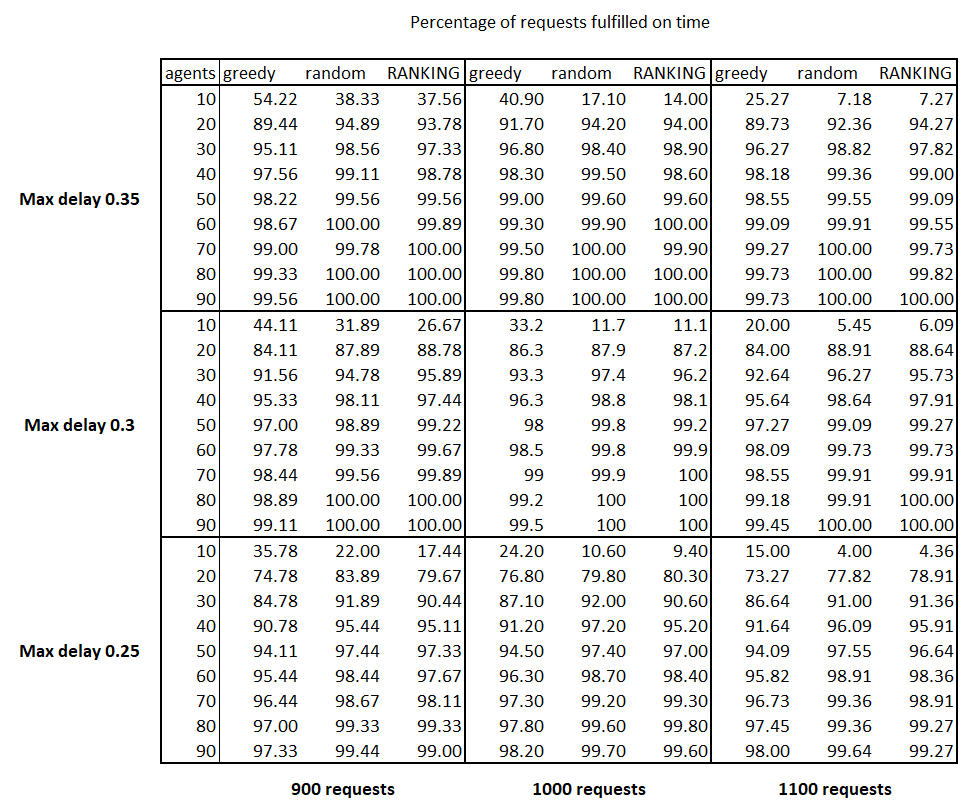
\includegraphics[scale = 0.9]{results}

We note that the greedy algorithm performs worse than the random and RANKING algorithms. Except for low-resource settings (low number of agents), where the percentage of requests fulfilled on time is unacceptably low anyway, the greedy algorithm has a consistently lower percentage of requests fulfilled on time compared to both the random and RANKING algorithms.

Correspondingly, the greedy algorithm would have a much higher minimum fleet size to guarantee that all requests are fulfilled on time. 

Also, from a preliminary view of the results, the difference in performance of the random and RANKING algorithm seems to be insignificant.

\subsection{Discussion}
While we did not expect that the greedy algorithm would perform consistently worse than the other algorithms, the results did agree with our expectation that the greedy algorithm is unlikely to perform better than the other algorithms.

The current implementation of the greedy algorithm tries to minimize the delay for each request. This greedy heuristic is more relevant to a problem that seeks to minimize average waiting time. However, as we aim to meet a maximum delay constraint, this heuristic is less applicable.

We note that the current implementation of the RANKING algorithm is unfeasible for real world application due to unfairness amongst the workers. We may modify the algorithm to change the ranks of workers after they are assigned to a task. We do not expect this to drastically affect the results, as the random algorithm seems to perform similarly to the current implementation of the RANKING algorithm.

\section{Plan for CP3209}
\label{sec:plan}
\subsection{Algorithms to Implement}
We intend to extend the prototype and study the performance of the following algorithms as well.

\subsubsection{Hybrid Greedy and RANKING}
An approach that could be studied is to apply the greedy algorithm on a subset of workers that can fulfill the request on time. This subset is created by taking the workers with the lowest ranks that can fulfill the request.

\subsubsection{A Different Greedy}
\label{heuristics}
As explained earlier, the greedy heuristic currently used is unsuitable for the minimum fleet problem. Here, we explore another heuristic that we could use.

The least location entropy priority introduced in section~\ref{llep} takes into account the frequency of past visitation as a proxy for distribution of crowdsourced workers. Under the context of the minimum fleet problem, location entropy itself is not completely relevant, given that the distribution of workers is known and volatile to assignments. However, informing our assignment with the current distribution of workers is a potential area to explore.

One way to do this is to measure worker density around each worker, by counting the number of workers that are within a certain distance to the worker of interest. A naive implementation of this would have a time complexity of $O(n^2)$ in the worst case. The direct use of worker density, however, may be less applicable in scenarios where locations are not distributed uniformly, and appropriate modifications have to be made.

Alternatively, we can select the worker with the lowest likelihood to be selected under a different algorithm (for example, the greedy algorithm)

Either way, the use of such methods requires further refining before implementation, and would likely require refactoring of the prototype to include additional data structures to efficiently perform experiments.

\subsubsection{Reserving Workers}
Another idea we can explore is to have strategically placed reserve workers that are only activated if the rest of the workers cannot fulfill the request on time. If there are non-reserve workers that can fulfill the task on time, we assign the non-reserve workers randomly.

This can be seen as a generalized version of the current implementation of the RANKING algorithm, as the reserve workers can be seen as the workers with the highest priority value in the RANKING algorithm, which are chosen only if the rest of the workers cannot fulfill the request on time.

To ensure strategic placement, we may have to move the reserve workers back to the original location at the start, and after any perturbations to the reserve workers. These modifications would require further changes to the prototype.

\subsection{Datasets}
\subsubsection{Generated Datasets}
\label{dataset}
We can expand the range of distributions of requests across location and time we study beyond the uniform distribution. Specifically, we can use the Normal, Power Law and Exponential distribution for the location of requests, similar to \cite{tong}. We can also modify the distribution of requests with a suitable multimodal distribution to account for peak periods.

\subsubsection{Real Datasets}
Similar to \cite{nature}, one of the real datasets we intend to use is the taxicab trip data in New York City, as the dataset is open, easily accessible, and spans over several years.

\subsubsection{Extending Real Datasets}
Using statistical analysis tools such as R, we can test for the goodness of fit of distribution of requests in real datasets over location or time, under the respective distributions mentioned in section~\ref{dataset}. If we manage to find a model that fits the real data, we can obtain the relevant parameters through maximum likelihood estimation and generate additional datasets.

\subsection{Extending to Graphs}
A major departure of our current prototype from the real world scenario is our representation of locations and distances. The Cartesian plane does not adequately capture networks for movement and transportation, which is best represented in a dynamic weighted graph.

We aim to move a step closer, by using a static weighted graph . We can explore techniques used by \cite{nature, preprocess} in constructing a graph representative of a real transportation network.

As an intermediate between these two representations, we may first implement a simple grid network structure to study the algorithms.

\subsection{Visualization}
A stretch goal of the project is to automate the visualization of each run of online task assignment, so that we can better understand how the algorithms perform through our visual observations.

\subsection{Timeline}
\subsubsection{Phase 1: OTA on Cartesian plane}
From November 2019 to December 2019, we aim to fully utilise the current prototype to analyse the performance of different algorithms over different distributions of location and time. 

By the end of December 2019, we aim to incorporate real datasets into the analysis. As a stretch goal, we aim to generate more datasets based on the real datasets as described above. However, this task takes a lower priority.

In this process, we will repeatedly analyse the results we obtain, using the minimum fleet size as well as percentage of requests fulfilled on time as performance metrics. We will then identify which algorithm is most suited for the minimum fleet problem.

\subsubsection{Phase 2: OTA on graphs}
Next, we aim to study the minimum fleet problem under a graph setting. This would require significant refactoring of the current prototype we are working with. We will verify if the algorithms examined in the previous phase have a similar performance in graphs. We hope to fully implement this by mid-February.

\bibliographystyle{nurop}
\bibliography{socreport}

\end{document}
